\documentclass[varwidth=true, border=2pt]{standalone}
\usepackage{tikz}

\begin{document}
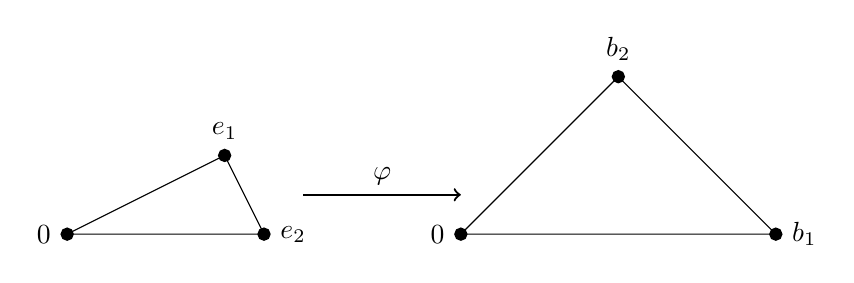
\begin{tikzpicture}
    \tikzstyle{point}=[circle,thick,draw=black,fill=black,inner sep=0pt,minimum width=4pt,minimum height=4pt]

    \node (a)[point,label={[label distance=0cm]180:$0$}] at (0,0) {};
    \node (b)[point,label={[label distance=0cm]0:$e_2$}] at (2.5,0) {};
    \node (c)[point,label={[label distance=0cm]90:$e_1$}] at (2,1) {};

    \begin{scope}[xshift=5cm]
        \node (d)[point,label={[label distance=0cm]180:$0$}] at (0,0) {};
        \node (e)[point,label={[label distance=0cm]0:$b_1$}] at (4,0) {};
        \node (f)[point,label={[label distance=0cm]90:$b_2$}] at (2,2) {};
    \end{scope}

    \draw (a.center) -- (b.center) -- (c.center) -- cycle;
    \draw (d.center) -- (e.center) -- (f.center) -- cycle;

    \draw[thick,->] (3,0.5) -- node[above] {$\varphi$} (5,0.5);
\end{tikzpicture}
\end{document}
